\documentclass{beamer}
 
\usepackage[utf8]{inputenc}
\usepackage{siunitx}
\usetheme{CambridgeUS}
\useinnertheme{circles}

\usefonttheme[onlymath]{serif} 
 
%Information to be included in the title page:

\title{Seminar 1}
\subtitle{Special relativity}

\author{Will Barker\inst{1}\inst{2}}
\institute{
  \inst{1}%
    Cavendish Laboratory\\
    University of Cambridge\\
  \inst{2}%
    Kavli Institute for Cosmology\\
    University of Cambridge\\
}
\date{}
\logo{%
  \makebox[0.95\paperwidth]{%
    
\includegraphics[height=0.7cm,keepaspectratio]{CU.eps}%
    \hfill%
    \includegraphics[height=0.7cm,keepaspectratio]{logo.png}%
  }%
}
 
 
 
\begin{document}
 
\frame{\titlepage}


\begin{frame}
  \frametitle{Calculus}
  \textit{[A quip] that the physicist Richard Feynman made to the novelist Herman Wouk when they were discussing the Manhattan Project. Wouk was doing research for a big novel he hoped to write about World War II, and he went to Caltech to interview physicists who had worked on the bomb, one of whom was Feynman. After the interview, as they were parting, Feynman asked Wouk if he knew calculus. No, Wouk admitted, he didn’t. “You had better learn it,” said Feynman. “It’s the language God talks.”}
\end{frame}

\begin{frame}
  \frametitle{Calculus}
  \begin{itemize}
    \item Before we do any physics we ought to talk about calculus and some special functions\ldots
  \end{itemize}
\end{frame}

\begin{frame}
  \frametitle{Calculus}
  \begin{itemize}
    \item<1-> Begin with a function, $y=f(x)$, basic statement of one variable depending on another
    \item<2-> Define the \textbf{derivative} of $y$ with respect to $x$
      <3->\begin{equation*}
	\frac{\mathrm{d}y}{\mathrm{d}x}=\lim_{\delta x\to 0}\frac{f(x+\delta x)-f(x)}{\delta x}
	\label{<+label+>}
      \end{equation*}
    \item<4-> This is a purely \textbf{formal} definition
    \item<5-> Don't get too hung up on what \textbf{differentials} $\mathrm{d}y$ and $\mathrm{d}x$ mean!
    \item<6-> Interpet it as the \textbf{rate of change} of $y$ with respect to $x$
  \end{itemize}
\end{frame}

\begin{frame}
  \frametitle{Calculus}
  \begin{itemize}
    \item<1-> Properties of differentiation:
      \begin{itemize}
	\item<2-> \textbf{Linearity}
	\item<3-> \textbf{Leibniz rule}
	\item<4-> \textbf{Chain rule}
      \end{itemize}
  \end{itemize}
\end{frame}

\begin{frame}
  \frametitle{Calculus}
  \begin{itemize}
    \item<1-> Simplest example, polynomial function:
      \begin{equation*}
	f(x)=c_0+c_1x+c_2x^2+c_3x^3+\cdots
	\label{<+label+>}
      \end{equation*}
    \item<2-> Take any term and apply the formula for differentiation:
      \begin{equation*}
	\frac{\mathrm{d}c_nx^n}{\mathrm{d}x}=\lim_{\delta x\to 0}\frac{c_n(x+\delta x)^n-c_nx^n}{\delta x}
      \end{equation*}
    \item<3-> Easy to then find derivatives of any polynomial by using the linearity property
  \end{itemize}
\end{frame}

\begin{frame}
  \frametitle{Calculus}
  \begin{itemize}
    \item<1-> The inverse operation is called \textbf{integration} and write it this way
      \begin{equation*}
	g(x)=\frac{\mathrm{d}f(x)}{\mathrm{d}x}\implies f(x)=\int g(x)\mathrm{d}x
	\label{<+label+>}
      \end{equation*}
    \item<2-> We have a formula to go from a function to its derivative, but \textbf{not} the other way around
    \item<3-> The only way to proceed is to \textbf{notice} that if $f(x)$ differentiates to $g(x)$, then it must be the correct answer!
  \end{itemize}
\end{frame}

\begin{frame}
  \frametitle{Calculus}
  \begin{itemize}
    \item<1-> Simplest example is to stick to polynomials and find f(x) such that:
      \begin{equation*}
	g(x)=4x^3, \quad f(x)=\int g(x)\mathrm{d}x
	\label{<+label+>}
      \end{equation*}
    \item<2-> We find
\begin{equation}
  f(x)=x^4+c
  \label{<+label+>}
\end{equation}
    \item<3-> The $+c$ part encodes the information lost in the process of differentiation, and we can see this from a discussion of \textbf{area under a curve}
  \end{itemize}
\end{frame}

\begin{frame}
  \frametitle{Calculus}
  \begin{itemize}
    \item<1-> Time to introduce a pair of very important functions
      \begin{equation*}
	\sin(x), \quad \cos(x)
      \end{equation*}
    \item<2-> These are the \textbf{trigonometric} functions
    \item<3-> Someone probably told you these have something to do with \textbf{triangles}, which is true but not so important in physics
    \item<4-> Equivalently, someone might have told you that these functions have something to do with waves, which is also not exactly wrong\ldots
  \end{itemize}
\end{frame}

\begin{frame}
  \frametitle{Calculus}
  \begin{itemize}
    \item<1-> Let's start with $\sin(x)$, we can see precisely what it is doing to $x$ by introducing the notion of a \textbf{power series}:
      \begin{equation*}
	\sin(x)=\sum_{n=0}^{\infty}\frac{(-1)^nx^{2n+1}}{(2n+1)!}
      \end{equation*}
    \item<2-> Don't be too concerned with this sigma and factorial notation, it translates to something very like a polynomial:
      \begin{equation*}
	\sin(x)=x-\frac{1}{6}x^3+\frac{1}{120}x^5-\frac{1}{5040}x^7+\cdots
	\label{<+label+>}
      \end{equation*}
    \end{itemize}
\end{frame}

\begin{frame}
  \frametitle{Calculus}
  \begin{itemize}
    \item<1-> Should be able to find the derivative of $\sin(x)$ quite easily, just apply the rules:
      \begin{equation*}
	\frac{\mathrm{d}\sin(x)}{\mathrm{d}x}=\sum_{n=0}^{\infty}\frac{(-1)^nx^{2n}}{(2n)!}
	\label{<+label+>}
      \end{equation*}
    \item<2-> By differentiating $\sin(x)$ we've stumbled on the definition of $\cos(x)$, what happens if we keep differentiating?
  \end{itemize}
\end{frame}

\begin{frame}
  \frametitle{Calculus}
  \begin{itemize}
    \item<1-> The \textbf{trigonometric} functions are how we rotate points in \textbf{three-dimensional space} (hence their application in triangles), we will touch on how to do this later, but $x$ just becomes the  \textbf{angle} of rotation
    \item<2-> There is another very similar pair of functions:
      \begin{equation*}
	\sinh(x), \quad \cosh(x)
      \end{equation*}
    \item<3-> These are known as the \textbf{hyperbolic} functions, they are used in the rotation of \textbf{four-dimensional space-time}
  \end{itemize}
\end{frame}

\begin{frame}
  \frametitle{Calculus}
  \begin{itemize}
    \item<1-> The \textbf{power series} for $\sinh(x)$ is as follows:
      \begin{equation*}
	\sinh(x)=\sum_{n=0}^{\infty}\frac{x^{2n+1}}{(2n+1)!}
	\label{<+label+>}
      \end{equation*}
    \item<2-> Once again a simple differentiation is sufficient to obtain $\cosh(x)$:
      \begin{equation*}
	\cosh(x)=\sum_{n=0}^{\infty}\frac{x^{2n}}{(2n)!}
	\label{<+label+>}
      \end{equation*}
    \item<3-> And this process continues in an obvious manner\ldots
  \end{itemize}
\end{frame}

\begin{frame}
  \frametitle{Calculus}
  \begin{itemize}
    \item<1-> The trigonometric and hyperbolic functions clearly have very similar power series and must be related
    \item<2-> To see how, we will need the \textbf{exponential} function:
      \begin{equation*}
	e^x
      \end{equation*}
    \item<3-> The number $e\approx 2.71828$ is known as \textbf{Euler's constant} -- this particular value enables us to write the following power series:
      \begin{equation*}
	e^x=\sum_{n=0}^{\infty}\frac{x^n}{n!}
      \end{equation*}
  \end{itemize}
\end{frame}

\begin{frame}
  \frametitle{Calculus}
  \begin{itemize}
    \item<1-> Now once again we want to differentiate this function to see what it gives:
      \begin{equation*}
	\frac{\mathrm{d}e^x}{\mathrm{d}x}=e^x
      \end{equation*}
    \item<2-> As with the trigonometric and hyperbolic functions, the exponential function emerges in all areas of physics, you have probably heard already that it describes \textbf{radioactive decay}, but also e.g. the behaviour of the size of the universe near its beginning (\textbf{inflation}) and end (\textbf{de-Sitter expansion})
  \end{itemize}
\end{frame}

\begin{frame}
  \frametitle{Calculus}
  \begin{itemize}
    \item<1-> The relation between the \textbf{exponential} and \textbf{hyperbolic} functions is fairly clear from the power series, we just need to get to grips with \textbf{even} and \textbf{odd} functions:
      \begin{equation}
	\sinh(x)=\frac{1}{2}\left( e^x-e^{-x} \right), \quad \cosh(x)=\frac{1}{2}\left( e^x+e^{-x} \right)
	\label{<+label+>}
      \end{equation}
    \item<2-> An obvious consequence of this is (known in mathematics as a \textbf{corollary}):
      \begin{equation*}
	e^x=\sinh(x)+\cosh(x)	
      \end{equation*}
    \item<3-> And another less obvious corollary:
      \begin{equation*}
	\cosh^2(x)-\sinh^2(x)=1
      \end{equation*}
  \end{itemize}
\end{frame}

\begin{frame}
  \frametitle{Calculus}
  \begin{itemize}
    \item<1-> The case of the \textbf{exponential} and \textbf{trigonometric} functions is a bit harder, we need to include \textbf{imaginary numbers} to account for all those strange $-1$ factors in the power series:
      \begin{equation*}
	i^2=-1
      \end{equation*}
    \item<2-> The only place we really unavoidably need imaginary (or \textbf{complex}) numbers is in \textbf{quantum mechanics} and its special-relativistic generalisation, \textbf{quantum field theory}
    \item<3-> However, keep in mind that physics only works because some fundamental quantities (i.e. \textbf{wavefunctions}) that describe real phenomena, can't be expressed using real numbers
  \end{itemize}
\end{frame}

\begin{frame}
  \frametitle{Calculus}
  \begin{itemize}
    \item<1-> We find:
      \begin{equation*}
	\sin(x)=\frac{1}{2i}\left( e^{ix}-e^{-ix} \right), \quad \cos(x)=\frac{1}{2}\left( e^{ix}+e^{-ix} \right)
      \end{equation*}
    \item<2-> Again there is a neat corollary to this:
      \begin{equation*}
	e^{ix}=\cos(x)+i\sin(x)
      \end{equation*}
    \item<3-> And something you have probably met before:
      \begin{equation*}
	\cos^2(x)+\sin^2(x)=1
      \end{equation*}
  \end{itemize}
\end{frame}

\begin{frame}
  \frametitle{Calculus}
  \begin{itemize}
    \item<1-> Before we move on to some physics, try differentiating the following:
      \begin{itemize}
	\item<2-> $x^2+5x^3+8$
	\item<3-> $\left( 3x^3+8x^8 \right)e^x$
	\item<4-> $\sin(x)\cos(x)$
	\item<5-> $\sin^2(x)\cos^2(x)$
      \end{itemize}
    \item<6-> Next, try these integrals:
      \begin{itemize}
	\item<7-> $\int \sin(x)\mathrm{d}x$
	\item<8-> $\int e^x\left( \sin(x)+\cos(x) \right)\mathrm{d}x$
	\item<9-> $\int x^5\left( \cosh(x)+\frac{1}{6}x\sinh(x) \right)\mathrm{d}x$
	\item<10> $\int e^{-x}\mathrm{d}x$
      \end{itemize}
  \end{itemize}
\end{frame}

\begin{frame}
  \frametitle{Calculus}
  \begin{itemize}
    \item<1-> Now apply the Leibniz and chain rules carefully when differentiating these:
      \begin{itemize}
	\item<2-> $\frac{x^2+5x^3+8}{\sin^2(x)\cos^2(x)}$
	\item<3-> $\cosh(\sin(e^{2x}))$
	\item<4-> $\sin(x+1)$
      \end{itemize}
  \end{itemize}
\end{frame}

\begin{frame}
  \frametitle{What is astrophysics?}
  \begin{itemize}
    \item $\uparrow$
    \item \textbf{An applied field of physics, so very messy!}
  \end{itemize}
\end{frame}

\begin{frame}
  \center
  \frametitle{Astrophysical phenomena}
  \includegraphics[height=5cm]{kepler_90.jpg}
\end{frame}

\begin{frame}
  \center
  \frametitle{Astrophysical phenomena}
  \includegraphics[height=5cm]{protoplanetary_disk.jpg}
\end{frame}

\begin{frame}
  \center
  \frametitle{Astrophysical phenomena}
  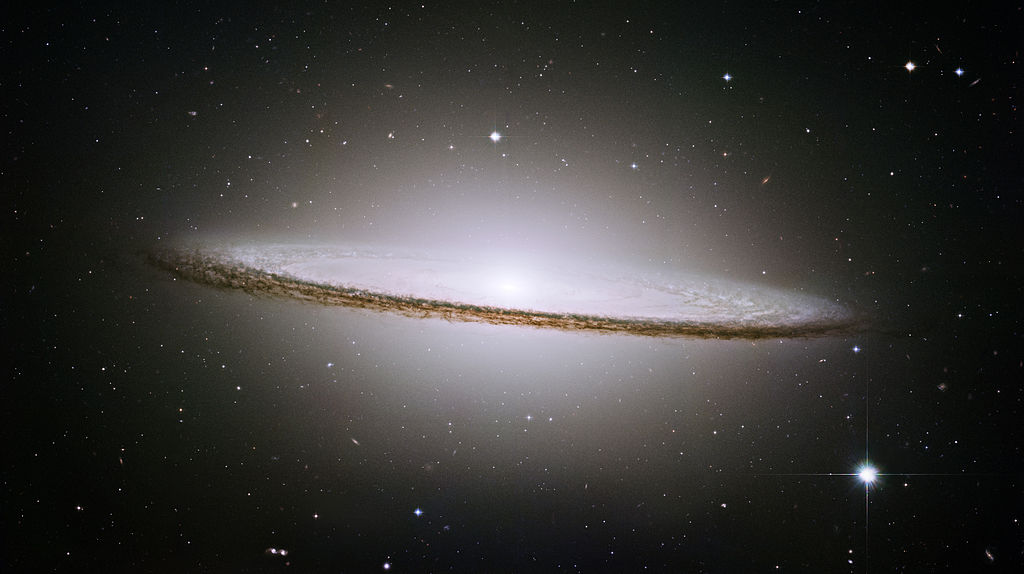
\includegraphics[height=5cm]{sombrero.jpg}
\end{frame}

\begin{frame}
  \center
  \frametitle{Astrophysical phenomena}
  \includegraphics[height=5cm]{m87.jpg}
\end{frame}

\begin{frame}
  \center
  \frametitle{Astrophysical phenomena}
  \includegraphics[height=5cm]{eht.jpg}
\end{frame}

\begin{frame}
  \center
  \frametitle{Astrophysical phenomena}
  \includegraphics[height=5cm]{hl_bh.jpg}
\end{frame}

\begin{frame}
  \center
  \frametitle{Astrophysical phenomena}
  \includegraphics[height=5cm]{gargantua.png}
\end{frame}

\begin{frame}
  \center
  \frametitle{Astrophysical phenomena}
  \includegraphics[height=5cm]{lensing.jpg}
\end{frame}

\begin{frame}
  \center
  \frametitle{Astrophysical phenomena}
  \includegraphics[height=5cm]{deep.jpg}
\end{frame}

\begin{frame}
  \center
  \frametitle{Astrophysical phenomena}
  \includegraphics[height=5cm]{cmb.jpg}
\end{frame}

\begin{frame}
  \center
  \frametitle{Astrophysical phenomena}
  \includegraphics[height=5cm]{big_bang.jpg}
\end{frame}

\begin{frame}
  \frametitle{Exoplanet miscellanea}
  \begin{itemize}
    \item We mentioned that transits were not so reliable:
      \includegraphics[height=4cm]{tabby.png}
  \end{itemize}
\end{frame}

\begin{frame}
  \frametitle{Exoplanet miscellanea}
  \begin{itemize}
    \item What is wrong with this light curve?
      \includegraphics[height=4cm]{tabby_2.jpg}
  \end{itemize}
\end{frame}

\begin{frame}
  \frametitle{Exoplanet miscellanea}
  \begin{itemize}
    \item Illustration of multiple \textbf{Dyson rings}:
      \includegraphics[height=4cm]{dyson.png}
  \end{itemize}
\end{frame}

\begin{frame}
  \frametitle{Exoplanet miscellanea}
  \begin{itemize}
    \item HabEx -- atmospheric backlighting in our own solar system:
      \includegraphics[height=4cm]{pluto_atmosphere.jpg}
  \end{itemize}
\end{frame}

\begin{frame}
  \frametitle{Exoplanet miscellanea}
  \begin{itemize}
    \item Which planet, if any?
      \includegraphics[height=4cm]{pluto.jpg}
  \end{itemize}
\end{frame}

\begin{frame}
  \frametitle{Exoplanet miscellanea}
  \begin{itemize}
    \item Solar coronograph:
      \includegraphics[height=4cm]{coronograph.png}
  \end{itemize}
\end{frame}

\begin{frame}
  \frametitle{Astrophysical scale}
  \begin{itemize}
    \item By definition, astrophysics will involve a wide range of \textbf{length scales}
  \end{itemize}
\end{frame}

\begin{frame}
  \frametitle{Astrophysical scale}
  \begin{itemize}
    \item Distance to space: \SI{1e2}{km}
  \end{itemize}
\end{frame}

\begin{frame}
  \frametitle{Astrophysical scale}
  \begin{itemize}
    \item Distance to the moon: \SI{4e5}{km}
  \end{itemize}
\end{frame}

\begin{frame}
  \frametitle{Astrophysical scale}
  \begin{itemize}
    \item Before we proceed further, we need to get to grips with the speed of light\ldots
  \end{itemize}
\end{frame}

\begin{frame}
  \frametitle{Astrophysical scale}
  \begin{itemize}
    \item The speed of light $c$ has the value \SI{3e8}{m/s}
    \item The earth has radius \SI{6.4e6}{m}, so how many times would light travel around the earth?
    \item The speed of light is \textbf{fixed}, it doesn't matter how you change you own velocity, $c$ will always give the same value upon measurement
  \end{itemize}
\end{frame}

\begin{frame}
  \frametitle{Astrophysical scale}
  \center
  \includegraphics[height=7cm]{mm.png}
\end{frame}

\begin{frame}
  \frametitle{Astrophysical scale}
  \begin{itemize}
    \item Counter-intuitively $c$ has \textbf{nothing} to do with light or electromagnetism, rather it is a unit-conversion between \textbf{space} and \textbf{time} -- which as we will see in Seminar 4 and 5, are the same thing
    \item Field theories (such as electromagnetism) have a mathematical structure such that (at the level of QFT) they contain \textbf{massless particles}
    \item \textbf{Special relativity} tells us that massless particles \textbf{always} move at $c$, or for every bit of time which elapses, they move through an \textbf{equal} bit of space
    \item \textbf{massive particles} (such as yourselves!) are free to move at any speed below $c$
  \end{itemize}
\end{frame}

\begin{frame}
  \frametitle{Astrophysical scale}
  \begin{itemize}
    \item Electromagnetism and quantum electrodynamics are not unique in that they contain massless \textbf{photons}
    \item Quantum chromodynamics (strong force) contains massless \textbf{gluons} and \textbf{classical} theories of gravity predict \textbf{gravitational waves} moving at $c$
    \item We expect that any quantum theory of gravity would therefore contain a massless \textbf{graviton}
  \end{itemize}
  \center
  \includegraphics[height=2cm]{gluon.png}
\end{frame}

\begin{frame}
  \frametitle{Astrophysical scale}
  \begin{itemize}
    \item \ldots back to astrophysics: because $c$ is so large, it is fairly useful for talking about scale
    \item The light minute: \SI{1.8e7}{km}
    \item The light year: \SI{9.5e12}{km}
    \item Clearly we are now talking about vast distances
  \end{itemize}
\end{frame}

\begin{frame}
  \frametitle{Astrophysical scale}
  \begin{itemize}
    \item Distance to the sun: \SI{8.5}{lm}
    \item Distance to the edge of the solar system: \SI{1}{ld}
    \item Let's pause here to define the \textbf{parsec}:
      \begin{itemize}
	\item The distance at which one \SI{1}{au} subtends one \textbf{arcsecond}
      \end{itemize}
  \end{itemize}
\end{frame}

\begin{frame}
  \frametitle{Astrophysical scale}
  \begin{itemize}
    \item Moving out\ldots
    \item Distance to Proxima Centauri: \SI{4.2}{ly}
    \item Distance to TRAPPIST-1: \SI{40}{ly}
    \item Distance to Sag A*: \SI{2.6e4}{ly}
    \item From this we get the length scale of our galaxy: \SI{1e4}{ly}
  \end{itemize}
\end{frame}

\begin{frame}
  \frametitle{Astrophysical scale}
  \begin{itemize}
    \item Since I mentioned Proxima b:
      \begin{itemize}
	\item https://www.youtube.com/watch?v=lysJduOqads 
	\item https://www.youtube.com/watch?v=RoCm6vZDDiQ
      \end{itemize}
  \end{itemize}
\end{frame}

\begin{frame}
  \frametitle{Astrophysical scale}
  \begin{itemize}
    \item Distance to LMC and SMC: \SI{1e5}{ly}
    \item Distance to Andromeda galaxy: \SI{2.5e6}{ly}
    \item Distance to M87: \SI{16.4e6}{pc}
  \end{itemize}
\end{frame}

\begin{frame}
  \frametitle{Astrophysical scale}
  \begin{itemize}
    \item Finally distance to the edge of the known universe: \SI{14e9}{pc}
  \end{itemize}
\end{frame}

\begin{frame}
  \frametitle{Astrophysical scale}
  \begin{itemize}
    \item Once we are in the realm of \SI{1e6}{pc} we should really be talking about \textbf{redshift}
    \item You will have heard about redshift in the context of fast-moving objects
    \item When we observe distant galaxies, we find that redshift \textbf{increases} with distance, and furthermore it does so \textbf{linearly} -- this is \textbf{Hubble's Law}
    \item However, to properly deal with these ideas we need \textbf{general relativity} -- effectively this replaces the notion of galaxies moving away with the idea of the space between expanding
    \item Before we cover general relativity, we need to tackle its little cousin\ldots
  \end{itemize}
\end{frame}

\begin{frame}
  \frametitle{Next topic\ldots}
  \center
  \includegraphics[height=5cm]{hyperspace.jpg}
\end{frame}
 
\begin{frame}
  \frametitle{What is special relativity?}
  \begin{itemize}
    \item<1-> Most importanty the \textbf{regime} $v\sim c$
    \item<2-> This regime tends to \textbf{break} classical laws of phyics:
      \begin{itemize}
	\item<3-> \textbf{quantum mechanics}\to\textbf{quantum field theory}
	\item<4-> \textbf{classical mechanics}\to\textbf{relativistic mechanics}
      \end{itemize}
    \item<5-> Three space dimensions and one time dimension are \textbf{aspects} of a connected whole known as \textbf{spacetime}
  \end{itemize}
\end{frame}

\begin{frame}
  \frametitle{Special vs general relativity}
  \begin{itemize}
    \item<1-> What is the difference between \textbf{special} and \textbf{general} relativity?
    \item<2-> \textbf{General relativity} is needed when there is enough \textbf{mass}, \textbf{energy}, \textbf{momentum} or \textbf{stress} (or when the \textbf{densities} of these are high enough) that there is some \textbf{gravity} involved
    \item<3-> What does that mean about the \textbf{shape} of spacetime?
      \begin{itemize}
	\item<4-> \textbf{Special relativity}\to\textbf{flat spacetime}
	\item<5-> \textbf{General relativity}\to\textbf{curved spacetime}
      \end{itemize}
  \end{itemize}
\end{frame}

\begin{frame}
  \frametitle{Special vs general relativity}
  \begin{itemize}
    \item<1-> The \textbf{three} dimensional space we all live in is known as \textbf{Euclidean} space
    \item<2-> \textbf{Euclidean} space has some properties you are all very \textbf{familiar} with, but which we need to describe \textbf{mathematically} in order to compare with \textbf{non-Euclidean} space (i.e. \textbf{four} dimensional spacetime):
      \begin{itemize}
	\item<3-> We can \textbf{rotate} the space
	\item<4-> We can define \textbf{distances} which don't change when we \textbf{rotate} the space
      \end{itemize}
  \end{itemize}
\end{frame}

\begin{frame}
  \frametitle{We want everything simple\ldots}
  \begin{itemize}
    \item<1-> We will only deal with \textbf{two} dimensions at a time, otherwise everything will become very complicated!
  \end{itemize}
\end{frame}

\begin{frame}
  \frametitle{Euclidean rotations}
  \begin{itemize}
    \item<1-> Start with \textbf{two} ordinary space dimensions and coordinates $x$ and $y$, what is a \textbf{vector} which describes a \textbf{position} in that space?
    \item<2-> Should have:
      \begin{align*}
	\mathbf{x}=
	\begin{bmatrix}
	  x\\
	  y
	\end{bmatrix}
      \end{align*}
  \end{itemize}
\end{frame}

\begin{frame}
  \frametitle{Euclidean rotations}
  \begin{itemize}
    \item<1-> Now we need to introduce \textbf{matrices}!
    \item<2-> Just a \textbf{table} of numbers:
      \begin{align*}
	\mathbf{R}=
	\begin{bmatrix}
	  a & b\\
	  c & d
	\end{bmatrix}
      \end{align*}
  \end{itemize}
\end{frame}

\begin{frame}
  \frametitle{Euclidean rotations}
  \begin{itemize}
    \item<1-> Now we \textbf{multiply} a \textbf{vector} by a \textbf{matrix}!
    \item<2-> Here is the \textbf{rule} for doing this:
      \begin{align*}
	\begin{bmatrix}
	  x'\\
	  y'
	\end{bmatrix}
	=
	\begin{bmatrix}
	  a & b\\
	  c & d
	\end{bmatrix}
	\begin{bmatrix}
	  x\\
	  y
	\end{bmatrix}
	=
	\begin{bmatrix}
	 ax+by\\
	 cx+dy
	\end{bmatrix}
      \end{align*}
    \item<3-> \textbf{WRITE THIS DOWN, YOU WILL NEED IT}
  \end{itemize}
\end{frame}

\begin{frame}
  \frametitle{Euclidean rotations}
  \begin{itemize}
    \item<1-> \textbf{Over to you}: find $x'$ and $y'$ if:
      \begin{align*}
	\mathbf{R}=
	\begin{bmatrix}
	  \hphantom{-}\cos(\theta) & \sin(\theta)\\
	  -\sin(\theta) & \cos(\theta)
	\end{bmatrix}
	, \quad
	\mathbf{x}=
	\begin{bmatrix}
	  1\\
	  0
	\end{bmatrix}
      \end{align*}
    \item<2-> (These names are recycled from the Program 1 students\ldots)
    \item<3-> Colin: $\theta=10^\circ$, Harry: $\theta=360^\circ$, Dylan: $\theta=45^\circ$, Jaazib: $\theta=70^\circ$, Ayush: $\theta=180^\circ$, Antonio: $\theta=270^\circ$, Nikolas: $\theta=280^\circ$, Thea: $\theta=290^\circ$, Naif: $\theta=-30^\circ$, Ilgin: $\theta=-40^\circ$, Francesco: $\theta=-90^\circ$
  \end{itemize}
\end{frame}

\begin{frame}
  \frametitle{Euclidean rotations}
  \begin{itemize}
    \item<1-> \textbf{Still over to you}: Now find $\sqrt{x'^2+y'^2}$ for these new vectors!
  \end{itemize}
\end{frame}

\begin{frame}
  \frametitle{Euclidean rotations}
  \begin{itemize}
    \item<1-> We should have found the following \textbf{exciting} things:
      \begin{itemize}
	\item<2-> The matrix \textbf{R} just \textbf{rotates} the position in space through the \textbf{angle}
	\item<3-> This leaves the \textbf{distance} from the origin \textbf{unchanged}
      \end{itemize}
  \end{itemize}
\end{frame}

\begin{frame}
  \frametitle{Euclidean rotations}
  \begin{itemize}
    \item<1-> So we can say this about \textbf{Euclidean} space:
      \begin{itemize}
	\item<2-> \textbf{Rotations} are done with \textbf{trigonometric} functions $\sin(\theta)$ and $\cos(\theta)$
	\item<3-> \textbf{Distances} are done like this: $\sqrt{x^2+y^2+z^2}$
      \end{itemize}
  \end{itemize}
\end{frame}

\begin{frame}
  \frametitle{Galilean rotations}
  \begin{itemize}
    \item<1-> This was rather \textbf{boring} actually, it gets more interesting if we have one \textbf{space} dimension and one \textbf{time} dimension
    \item<2-> It would be nice if we could set up this \textbf{two} dimensional space with coordinates which have the same \textbf{units}
    \item<3-> Let's say \textbf{space} is just given by $x$, what would be a good coordinate for time?
    \item<4-> So our new \textbf{position vector} is:
      \begin{align*}
	\mathbf{x}=
	\begin{bmatrix}
	  ct\\
	  x
	\end{bmatrix}
      \end{align*}
  \end{itemize}
\end{frame}

\begin{frame}
  \frametitle{Galilean rotations}
  \begin{itemize}
    \item<1-> We've just started to put together the idea of \textbf{spacetime}!
    \item<2-> Some important points:
      \begin{itemize}
	\item In \textbf{space} positions are usually known as \textbf{points}
	\item In \textbf{spacetime} the positions are known as \textbf{events}
      \end{itemize}
    \item<3-> Why?
  \end{itemize}
\end{frame}

\begin{frame}
  \frametitle{Galilean rotations}
  \begin{itemize}
    \item<1-> Now things begin getting complicated\ldots
    \item<2-> Let's say we start moving along the $x$ direction at \textbf{constant} velocity $v$ (couldn't think of a simpler motion really\ldots)
    \item<3-> At $t=0$, we were at $x=0$
    \item<4-> What is our $x$ at general $t$?
  \end{itemize}
\end{frame}

\begin{frame}
  \frametitle{Galilean rotations}
  \begin{itemize}
    \item<1-> Now things begin getting complicated\ldots
    \item<2-> Let's say we start moving along the $x$ direction at \textbf{constant} velocity $v$ (couldn't think of a simpler motion really\ldots)
    \item<3-> At $t=0$, we were at $x=0$
    \item<4-> What is our $x$ at general $t$?
    \item<4-> What is our $t$ at general $t$ (trick question!)?
  \end{itemize}
\end{frame}

\begin{frame}
  \frametitle{Galilean rotations}
  \begin{itemize}
    \item<1-> With this in mind, how will we measure $t'$ and $x'$ of some \textbf{event}:
      \begin{align*}
	\mathbf{x}=
	\begin{bmatrix}
	  ct\\
	  x
	\end{bmatrix}
      \end{align*}
    \item<2-> Just using common sense, we should end up with these very simple formulae:
      \begin{gather*}
	t'=t,\\
	x'=x-vt
      \end{gather*}
  \end{itemize}
\end{frame}

\begin{frame}
  \frametitle{Galilean rotations}
  \begin{itemize}
    \item<1-> These are the formulae for \textbf{Galilean} transformations:
      \begin{gather*}
	t'=t,\\
	x'=x-vt
      \end{gather*}
    \item<2-> You all already \textbf{knew these}: they just say that if you \textbf{move}, the \textbf{time} you observe an event is \textbf{the same}, but the position of the event \textbf{moves toward you} (or away if $v\to -v$)
    \item<3-> Does anyone \textbf{disagree}?
    \item<4-> These formulae are \textbf{completely and utterly wrong}, but nobody noticed until 1905!
  \end{itemize}
\end{frame}

\begin{frame}
  \frametitle{Galilean rotations}
  \begin{itemize}
    \item<1-> Note that I used the word \textbf{transformations} for $t\to t'$ and $x\to x'$, but \textbf{rotations} for $x\to x'$ and $y\to y'$
    \item<2-> That is because the idea of \textbf{rotating space} makes \textbf{perfect sense}, but \textbf{rotating space and time} sounds like \textbf{nonsense}\ldots
    \item<3-> Let's do it anyway!
  \end{itemize}
\end{frame}

\begin{frame}
  \frametitle{Lorentz rotations}
  \begin{itemize}
    \item<1-> \textbf{Over to you again}: find $t'$ and $x'$ if:
      \begin{align*}
	\mathbf{R}=
	\begin{bmatrix}
	  \frac{1}{\sqrt{1-v^2/c^2}} & \frac{-v/c}{\sqrt{1-v^2/c^2}}\\
	  \frac{-v/c}{\sqrt{1-v^2/c^2}} & \frac{1}{\sqrt{1-v^2/c^2}}
	\end{bmatrix}
	, \quad
	\mathbf{x}=
	\begin{bmatrix}
	  ct\\
	  x
	\end{bmatrix}
	=
	\begin{bmatrix}
	  1\\
	  0
	\end{bmatrix}
      \end{align*}
    \item<2-> Again, the names are from the last group\ldots
    \item<2-> Colin: $v=c$, Harry: $v=2c$, Dylan: $v=0$, Jaazib: $v=0.5c$, Ayush: $v=0.2c$, Antonio: $v=0.1c$, Nikolas: $v=-0.1c$, Thea: $v=0.1c$, Naif: $v=-0.8c$, Ilgin: $v=-0.3c$, Francesco: $v=0.1c$
  \end{itemize}
\end{frame}

\begin{frame}
  \frametitle{Lorentz rotations}
  \begin{itemize}
    \item<1-> \textbf{Next task}: find $\sqrt{c^2t'^2-x'^2}$ for your vectors!
  \end{itemize}
\end{frame}

\begin{frame}
  \frametitle{Lorentz rotations}
  \begin{itemize}
    \item<1-> \textbf{Now find this}:
      \begin{equation*}
	\left( \frac{1}{\sqrt{1-v^2/c^2}} \right)^2-\left( \frac{-v/c}{\sqrt{1-v^2/c^2}} \right)^2
      \end{equation*}
    \item<2-> \textbf{Finally who can remember what this is} for any $\psi$:
      \begin{equation*}
	\cosh(\psi)^2-\sinh(\psi)^2
      \end{equation*}
    \item<3-> Claudia: $\psi$ is another Greek letter pronounced `psi' ;) 
  \end{itemize}
\end{frame}

\begin{frame}
  \frametitle{Lorentz rotations}
  \begin{itemize}
    \item<1-> So it turns out we can just write that horrible matrix in a simple form:
      \begin{align*}
	\mathbf{R}=
	\begin{bmatrix}
	  \frac{1}{\sqrt{1-v^2/c^2}} & \frac{-v/c}{\sqrt{1-v^2/c^2}}\\
	  \frac{-v/c}{\sqrt{1-v^2/c^2}} & \frac{1}{\sqrt{1-v^2/c^2}}
	\end{bmatrix}
	=
	\begin{bmatrix}
	  \cosh(\psi) & \sinh(\psi)\\
	  \sinh(\psi) & \cosh(\psi)
	\end{bmatrix}
	=\mathbf{\Lambda}
      \end{align*}
    \item<2-> Claudia: $\Lambda$ is uppercase Greek letter `lambda', lowercase is $\lambda$ ;) 
  \end{itemize}
\end{frame}

\begin{frame}
  \frametitle{Lorentz rotations}
  \begin{itemize}
    \item<1-> So unlike last time, the things we get now should actually be interesting:
      \begin{itemize}
	\item<2-> When we move, space and time \textbf{rotate}, but instead of \textbf{trigonometric} rotations with $\sin(\theta)$ and $\cos(\theta)$ for some angle $\theta$ we have \textbf{hyperbolic} rotations with \textbf{hyperbolic} functions $\sinh(\psi)$ and $\cosh(\psi)$ -- don't bother with what $\psi$ actually is, there is a formula for it in terms of $v/c$ (Mason, find $\psi(v/c)$)
	\item<3-> The \textbf{distance} in spacetime is just $\sqrt{c^2t^2-x^2-y^2-z^2}$
      \end{itemize}
  \end{itemize}
\end{frame}

\begin{frame}
  \frametitle{Lorentz rotations}
  \begin{itemize}
    \item<1-> Some long words:
      \begin{itemize}
	\item<2-> \textbf{Distance} in spacetime is known as the \textbf{interval} -- in the same sense that the \textbf{point} is known as an \textbf{event}
	\item<3-> We did \textbf{trigonometric} rotations in \textbf{Euclidean space} -- the space we live in -- these \textbf{hyperbolic} rotations are in \textbf{Minkowskian spacetime}
	\item<4-> \textbf{Minkowskian spacetime} is flat, but has a \textbf{negative metric signature} -- soon we will look at general relativity, in which the metric signature is the same, but because there is \textbf{gravity} the spacetime is \textbf{curved}
	\item<5-> You might want to look up some of these terms, but we don't have time (or the methematical development) to go into them
      \end{itemize}
  \end{itemize}
\end{frame}

\begin{frame}
  \frametitle{Lorentz rotations}
  \begin{itemize}
    \item<1-> Note to self: find some Lorentz transformations on Youtube
  \end{itemize}
\end{frame}

\begin{frame}
  \frametitle{Lorentz rotations}
  \begin{itemize}
    \item<1-> But I didn't go into why any of this \textbf{hyperbolic/Lorentz} rotation stuff is true\ldots
    \item<2-> In fact, we were happy with the simpler Galilean transformations before weren't we?
    \item<3-> Go back to $t$ and $x$ (i.e. \textbf{two dimensional case}) -- what if the \textbf{event} was a photon being \textbf{emitted} in the past at $t<0$ and some position $x$, and detected by us ($v=0$) at the \textbf{origin} of spacetime ($t_0=0$ and $x_0=0$) \textbf{Find the interval for the photon}:
      \begin{equation*}
	\sqrt{c^2t^2-x^2}
      \end{equation*}
  \end{itemize}
\end{frame}

\begin{frame}
  \frametitle{Lorentz rotations}
  \begin{itemize}
    \item<1-> We should find:
      \begin{equation*}
	\sqrt{c^2t^2-x^2}=0
      \end{equation*}
    \item<2-> This relies on the photon moving at $c$, right?
    \item<3-> And even if we start moving at $v$ we just spent ages proving that the \textbf{interval} of the photon's motion remains \textbf{unchanged}:
      \begin{equation*}
	\sqrt{c^2t'^2-x'^2}=0
      \end{equation*}
    \item<4-> So when we are moving at $v$, \textbf{what is the speed of the photon}?
    \item<5-> So all this \textbf{hyperbolic} rotation stuff just ensures that \textbf{the speed of light is the same, no matter how fast you are moving}
  \end{itemize}
\end{frame}

\begin{frame}
  \frametitle{Lorentz rotations}
  \begin{itemize}
    \item<1-> Finally, we can note the \textbf{Lorentz} rotations:
      \begin{gather*}
	ct'=\frac{ct}{\sqrt{1-v^2/c^2}}-\frac{vx/c}{\sqrt{1-v^2/c^2}},\\
	x'=\frac{x}{\sqrt{1-v^2/c^2}}-\frac{vt}{\sqrt{1-v^2/c^2}},
      \end{gather*}
    \item<2-> And \textbf{Galilean} transformations:
      \begin{gather*}
	t'=t,\\
	x'=x-vt,
      \end{gather*}
    \item<3-> \textbf{Explain why Galilean transformations are okay so long as} $v\ll c$
  \end{itemize}
\end{frame}

\begin{frame}
  \frametitle{Lorentz rotations}
  \begin{itemize}
    \item<1-> We also have \textbf{relativistic} momentum:
      \begin{gather*}
	p=\frac{mv}{\sqrt{1-v^2/c^2}}
      \end{gather*}
    \item<2-> And \textbf{non-relativistic} momentum:
      \begin{gather*}
	p=mv
      \end{gather*}
    \item<3-> \textbf{Explain why they agree at} $v\ll c$
  \end{itemize}
\end{frame}

\begin{frame}
  \frametitle{Lorentz rotations}
  \begin{itemize}
    \item<1-> Finally we have \textbf{relativistic} energy:
      \begin{gather*}
	\mathcal{  E}=\frac{mc^2}{\sqrt{1-v^2/c^2}}
      \end{gather*}
    \item<2-> \textbf{What happens at} $v\ll c$?
    \item<3-> Should have \textbf{non-relativistic} energy:
      \begin{gather*}
	\mathcal{  E}\approx mc^2+\frac{1}{2}mv^2
      \end{gather*}
  \end{itemize}
\end{frame}

\begin{frame}
  \frametitle{Lorentz rotations}
  \begin{itemize}
    \item<1-> Should have \textbf{non-relativistic} energy:
      \begin{gather*}
	\mathcal{  E}\approx mc^2+\frac{1}{2}mv^2
      \end{gather*}
    \item<2-> What happens if the particle is standing still?
      \begin{equation*}
	\mathcal{  E}=mc^2
      \end{equation*}
    \item<3-> \textbf{The end.}
  \end{itemize}
\end{frame}

\begin{frame}
  \center
  \frametitle{Astrophysical phenomena}
  \includegraphics[height=5cm]{einstein.jpg}
\end{frame}

\end{document}


